%TODO: rewrite
%TODO: reduce total number of todos
%TODO: add paragraph about xetal-pro from preparation

\begin{figure}[t]
\centering
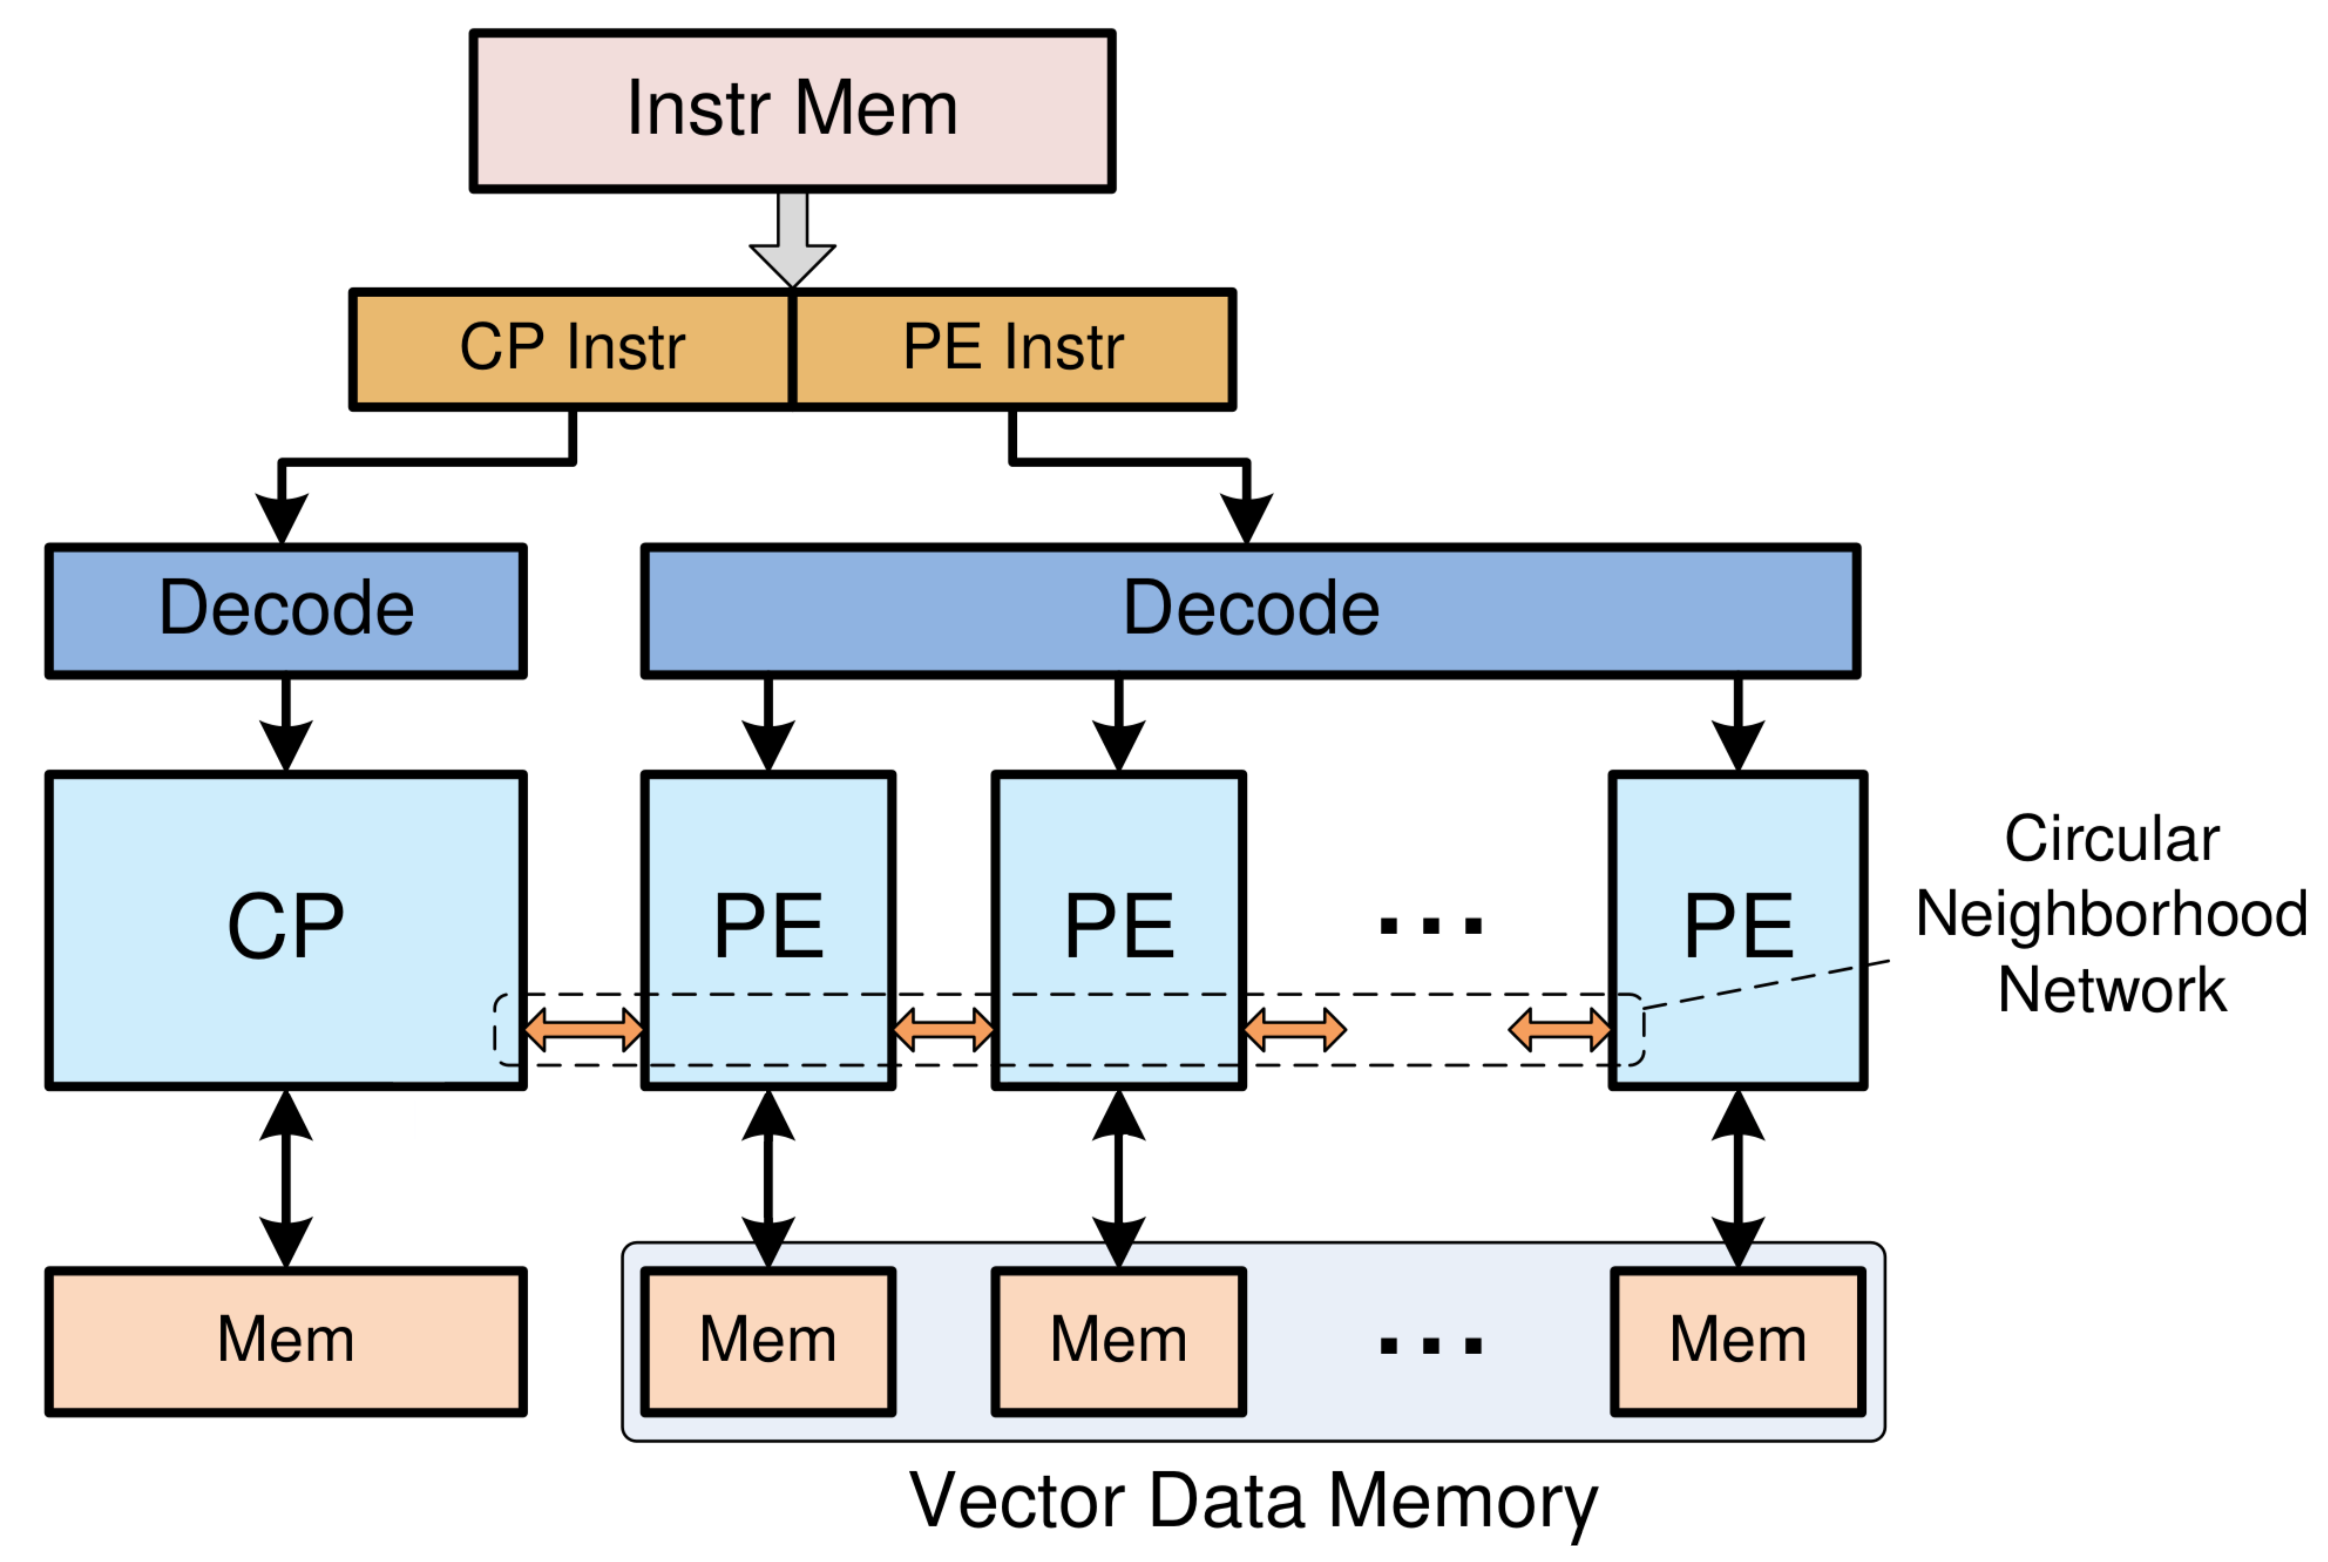
\includegraphics[width=.6\textwidth]{figures/simd_overview}
\caption{General overview of the wide SIMD architecture.}
\label{fig:simd_overview}
\end{figure}

The advantage of the SIMD architecture is that multiple operations are processed in parallel instead of processing them in a sequence. Therefore, the same performance can be achieved at a much lower clock frequency, thereby reducing voltage and thus energy consumption \cite{dongrio1}. Furthermore, because each Processing Element (PE) executes the same instruction, the Instruction Fetch (IF) and Instruction Decode (ID) can be shared amongst the PEs, reducing energy consumption.

We propose a wide SIMD architecture \cite{simd} that performs wide vector operations that exploit DLP by executing the same instruction on multiple data simultaneously. Figure \ref{fig:simd_overview} shows a general overview of the SIMD processor.
We have one Control Processor (CP) responsible for scalar operations and control flow i.e. jump/branch instructions. Furthermore, there is a wide array of PEs responsible for processing vector operations. The CP executes in parallel with the PEs, exploiting ILP.

The proposed architecture has a Reduced Instruction Set Computer (RISC) Instruction Set Architecture (ISA) that is divided up into three categories of instructions. In general, instructions have two operands and a destination register. Instructions that take two register files as operands are Register-type (R-type) instructions. Instructions that take a register file and an immediate as operands are called Immediate-type (I-type). The control flow can be controlled by using Jump-type (J-type) instructions, which can only be executed by the CP.

\begin{figure}[b!]
\centering
\subfloat[Datapath with implicit bypassing.]{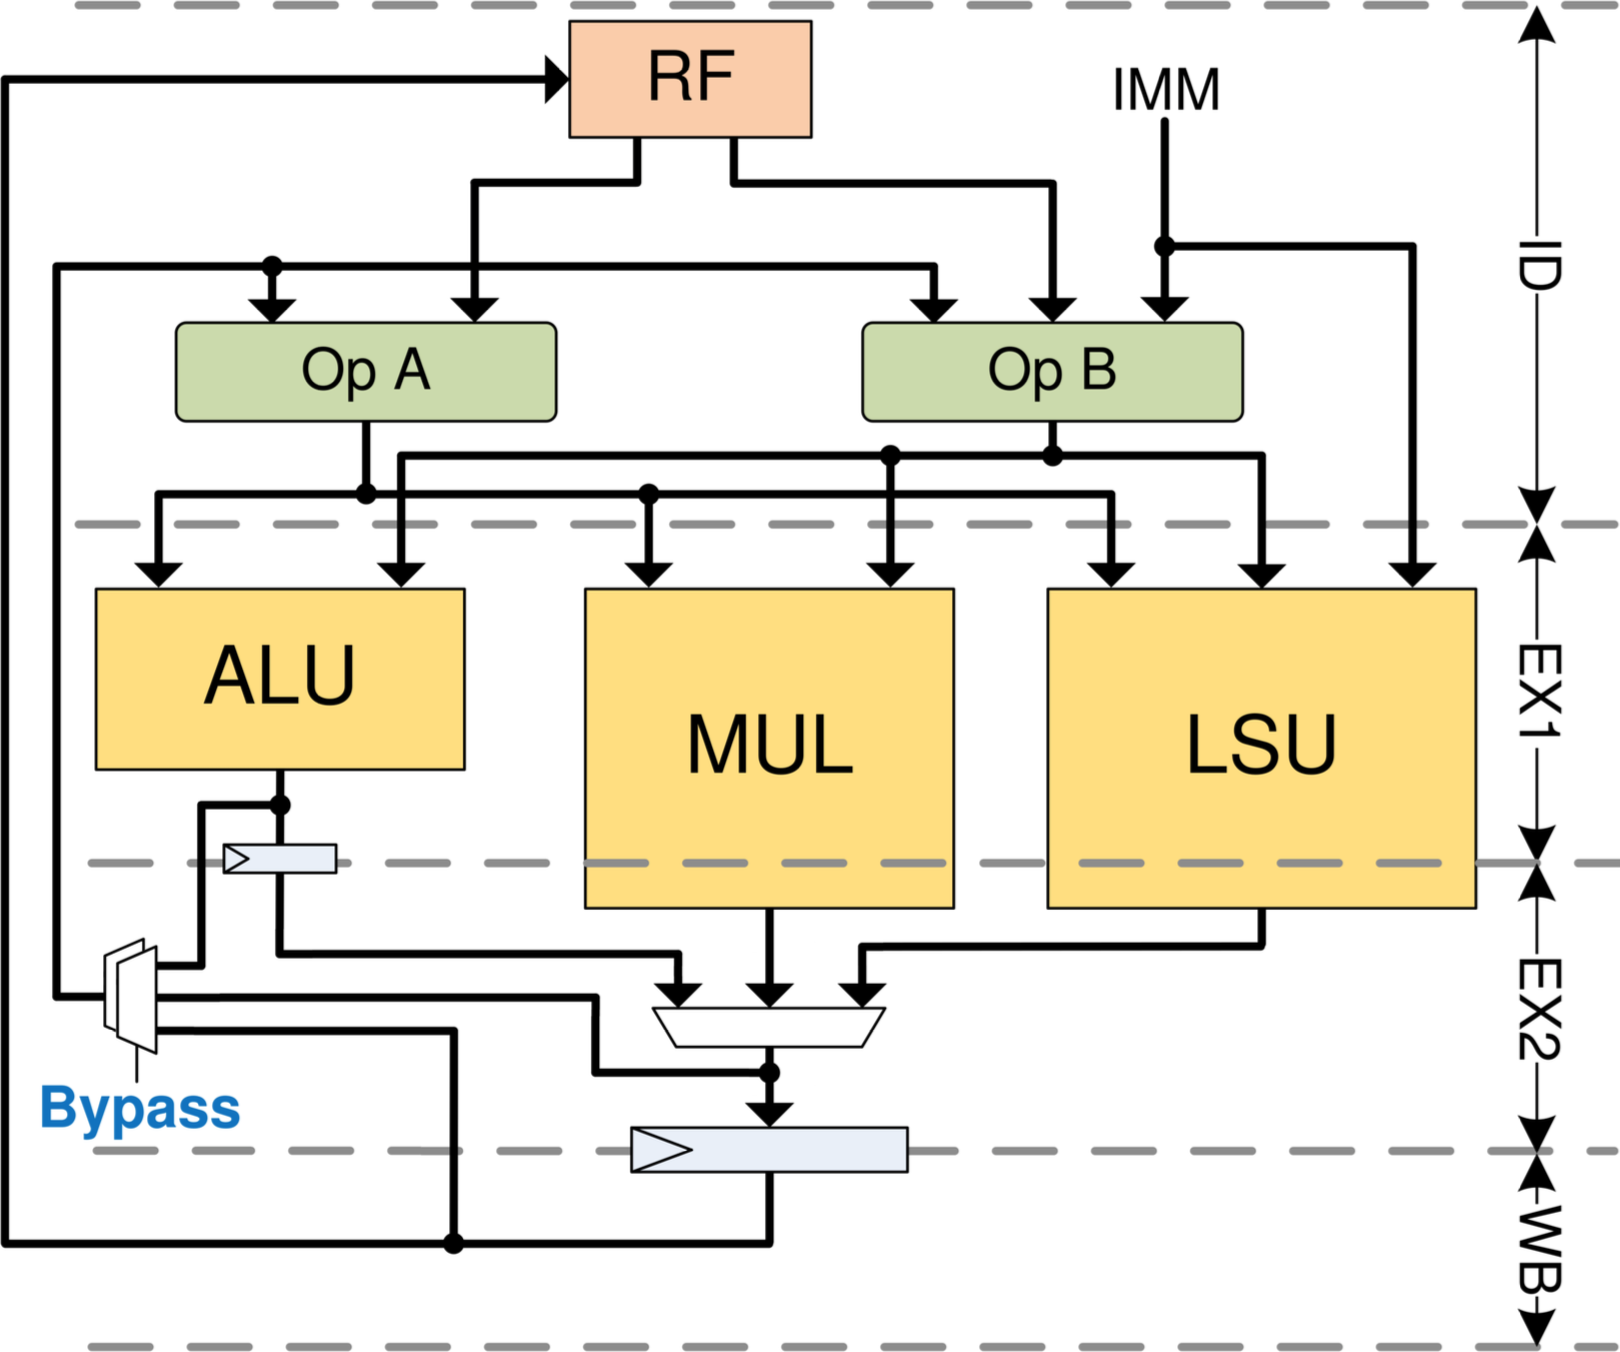
\includegraphics[width=.475\textwidth]{figures/transparent_bypass}%
\label{fig:transparent_datapath}}
\hfil
\subfloat[Datapath with explicit bypassing.]{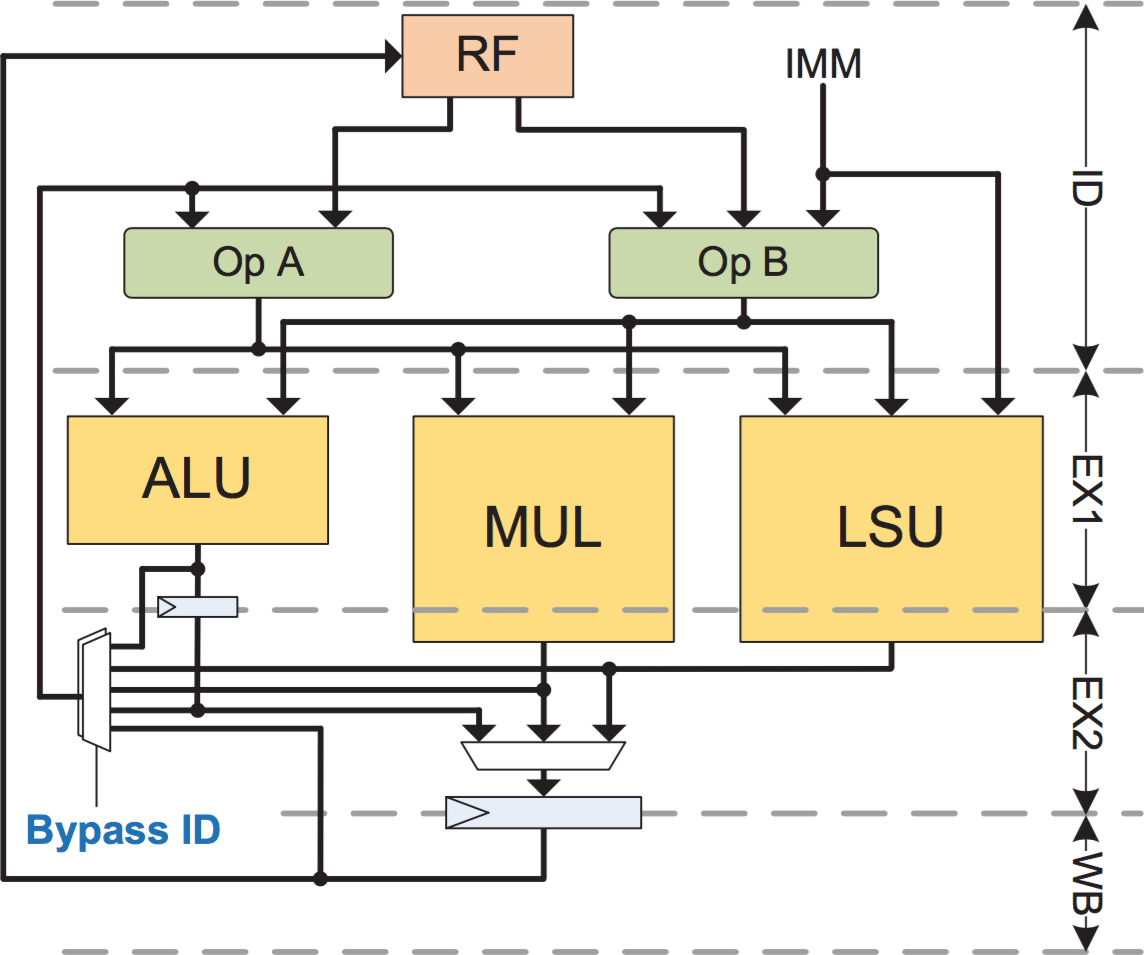
\includegraphics[width=.475\textwidth]{figures/explicit_bypass}%
\label{fig:explicit_datapath}}
\caption{Bypassing network differences between implicit bypassing and explicit bypassing.}
\label{fig:datapath_approaches}
\end{figure}

%TODO: add here that we have in general an iF, ID, one or more EX and a wb stages and that normally the result is not available until after the wb stageis complete, but with bypassing, whether it is transparent or explicit bypassing, we can get the result at an earlier stage. 

As an extra challenge for the compiler, the architecture is designed to be configurable, e.g. width of the PE array, bit width of the wires and registers, the number of stages that the instruction pipeline consists of, and whether it has implicit or explicit bypassing, can be configured. The data width of the wires and registers can be configured into 16-bits or 32-bits.

In order to support a configurable number of PE elements, a neighbourhood network topology is chosen for its scalability. With a circular neighbourhood network topology, the connection between the first and last PE does not introduce extra long wires, because the PEs can be placed in a circular manner \cite{dongrio2}.

%=============================== NN speech ===============================
%\section{Neighbourhood Network}\label{sec:nn}
%Each processor (CP or PE) does not only execute independently, but can also exchange data with its direct neighbours. However, because we have limited connectivity, moving data from one PE to another PE can introduce additional cycles. Namely, when communicating with non-direct neighbours. The circular neighbourhood network that is used to connect the processors is illustrated in Figure \ref{fig:neighborhood_network}. The CP can select data from the first and last PE, and each PE can communicate with its direct neighbours, or (not illustrated in Figure \ref{fig:neighborhood_network}) receive data from the CP by means of a broadcast.

%\begin{figure}[H]
%\centering
%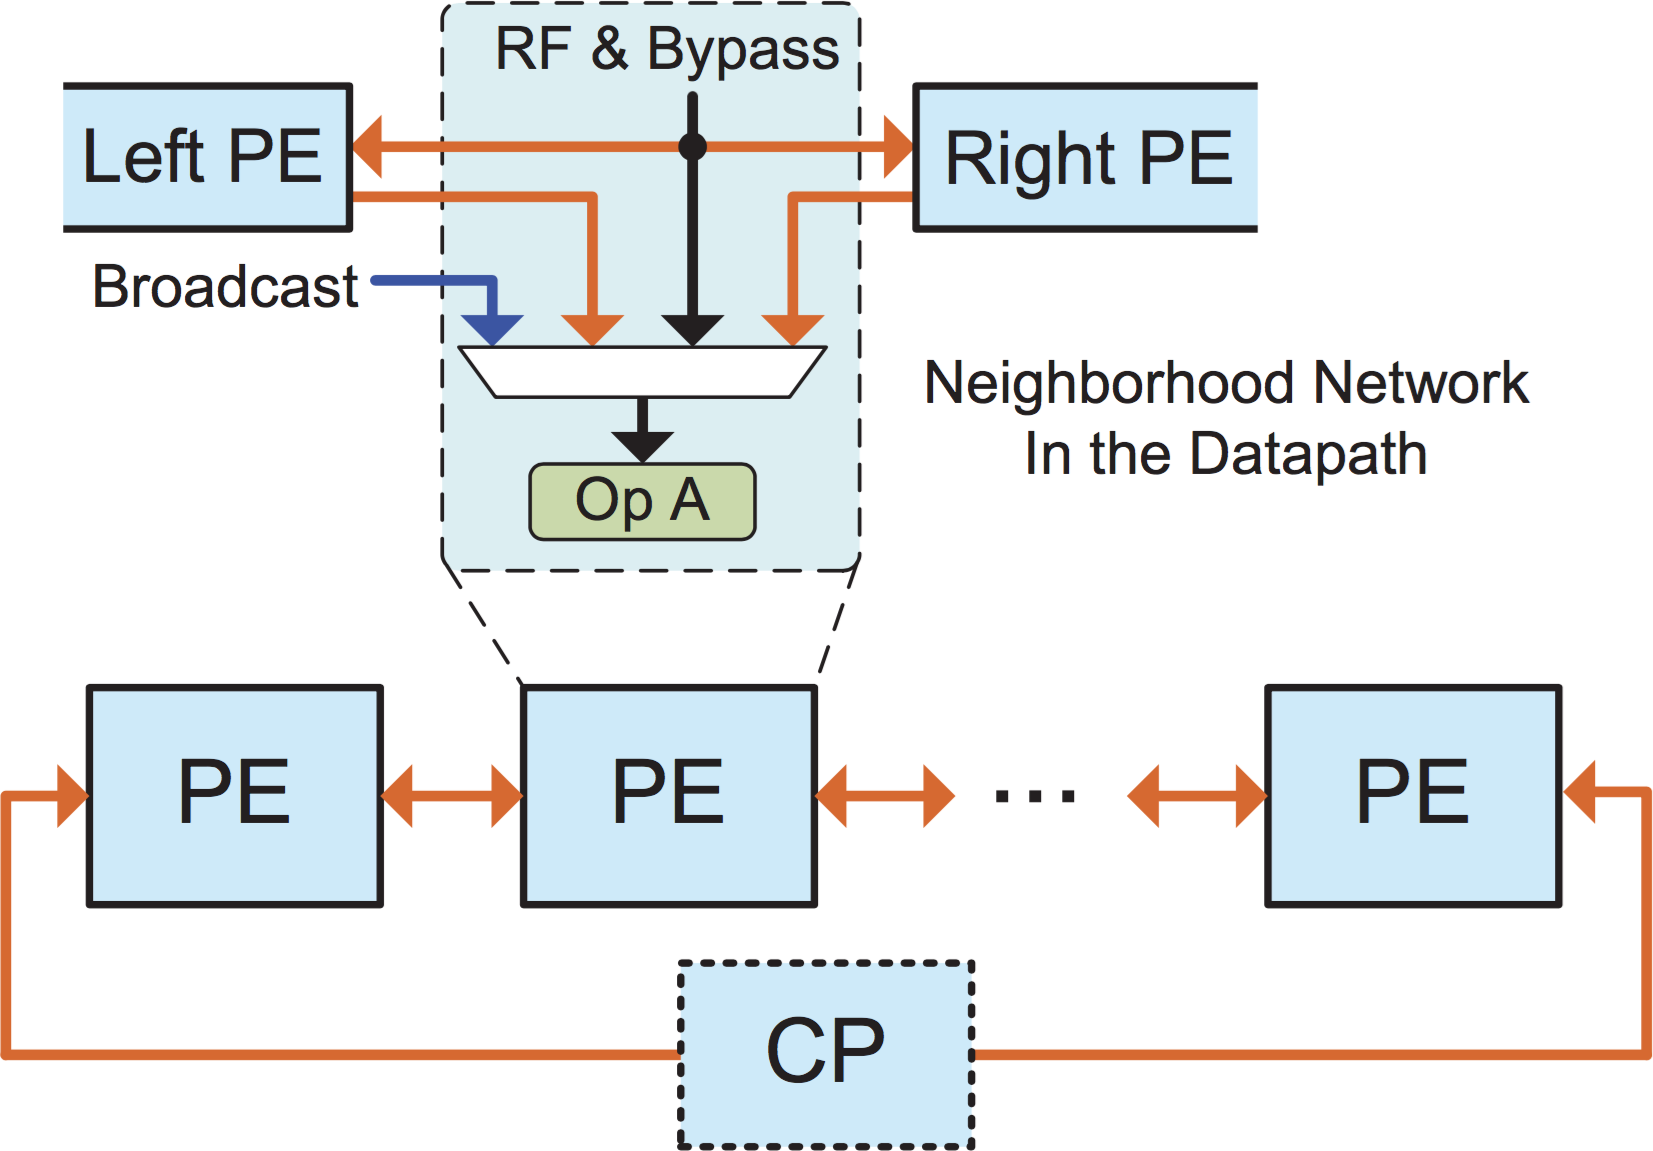
\includegraphics[width=.4\textwidth]{figures/neighborhood_network}
%\caption{Illustration of the circular neighborhood network.}
%\label{fig:neighborhood_network}
%\end{figure}

%The processor selects data from its neighbours in the instruction decode stage. Depending on the "select data" bits, it either takes data from one of its neighbours or from itself. Table \ref{table:select_data} gives an overview of the communication mode, depending on the value of "select data". The "select data" bits are decoded in each instruction, as we will show in Chapter \ref{sec:isa}.
 
% \begin{table}[H]
%\caption{Communication model for the CP and PEs, depending on the value of "select data".}
%\begin{center}
%\begin{tabular}{|c|c|c|}
%\hline
%\textbf{select data} & \textbf{CP} & \textbf{PE} \\ \hline
%2'b00 & Select data from \emph{self}. & Select data from \emph{self}. \\ \hline
%2'b01 & Select data form \emph{last} PE. & Select data from \emph{right} neighbour. \\ \hline
%2'b10 & Select data from \emph{first} PE. & Select data from \emph{left} neighbour. \\ \hline
%2'b11 & Not used. & Select data from CP \emph{broadcast}. \\ \hline
%\end{tabular}
%\end{center}
%\label{table:select_data}
%\end{table}%

%The processors communicate with each other by writing directly to the output of the operand register based on the values of bits "select data" bits. When the value of these two bits is $00$, data is selected from the processor itself. When these bits are $01$, data is selected from the last PE, in case of the CP executing this instruction, and from the right neighbour in case of a PE executing this instruction. Similarly, having a value of $10$, data is selected from the first PE in case of the CP executing this instruction, or left neighbour in case of a PE is executing this instruction. Finally, a value of $11$ will select data from the CP broadcast in the case that a PE is executing the instruction.

%=============================== Datapath speech ===============================
\subsection{Processor Pipeline and Datapath}\label{sec:processor}
%TODO: make new pictures for difference 4 and 5 stage without all difficult information
\begin{figure}[b!]
\centering
\subfloat[4-stage pipeline processor overview.]{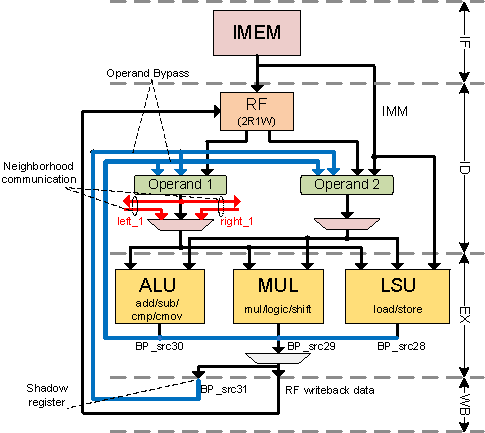
\includegraphics[width=.475\textwidth]{figures/4-stage_bypass}%
\label{fig:4_stage}}
\hfil
\subfloat[5-stage pipeline with processor overview.]{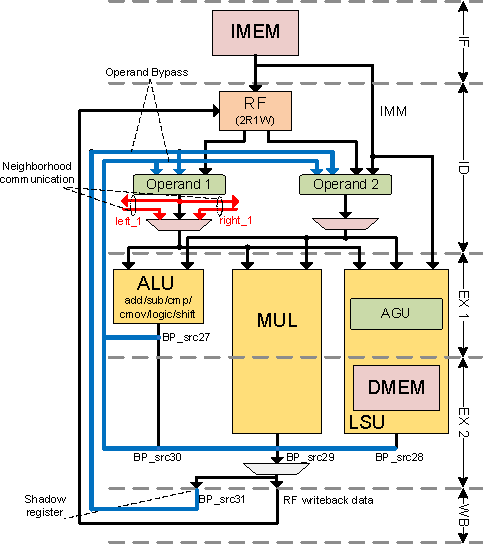
\includegraphics[width=.475\textwidth]{figures/5-stage_bypass}%
\label{fig:5_stage}}
\caption{Bypassing network differences between four stage and five stage pipeline configuration.}
\label{fig:datapath_pipeline_conf}
\end{figure}
%TODO: Write new paragraph about.general layout

Generally, each processor (CP or PE) has its own registers and three functional units, i.e. ALU, MUL and LSU. 

The instruction pipeline is divided up into four or five stages. Top down, we have an IF-stage, an ID-stage, one or more execution stages and a Write Back (WB) stage. The architecture shown in Figure \ref{fig:4_stage} has four stages while the architecture shown in Figure \ref{fig:5_stage} has five stages.

The neighbourhood communication network is implemented by overriding the output of $operand\ 1$ in ID-stage. Depending on the decoded instruction, data is either selected from another (neighbouring) processor, from the local RF or from the bypass network. Each FU has private input registers, which keep the result at the output of a compute unit valid as long as no new operation or input is assigned to it \cite{dongrio1}. The outputs can be used in the bypass network to bypass any of the operands in an instruction. This \emph{operand isolation} reduces toggling in the FUs, and creates extra opportunities for bypassing.

We can configure the SIMD to have either explicit or implicit bypassing. With implicit bypassing, also called transparent bypassing it is the hardware's responsibility to handle bypassing. With explicit bypassing, on the other hand, the bypasses are encoded in the instructions, and it is thus the compiler's responsibility to handle bypassing.

%We can configure the SIMD to have four or five stages. With four stages shown in Figure \ref{fig:4_stage}, all instructions take a single cycle, while with the five stages shown in Figure \ref{fig:5_stage}, ALU takes a single cycle, while MUL and LSU take two cycles, as shown in Table \ref{table:FU_cycles}. With 5 stages, MUL takes twice as many cycles. However, additions are simpler to perform, therefore the efficiency. 

%\begin{table}[H]
%\caption{Cycles per FU.}
%\begin{center}
%\begin{tabular}{|c|c|c|}
%\hline & \multicolumn{2}{c|}{\textbf{Cycles}} \\ \hline
%\textbf{FU} & \textbf{4-stage} & \textbf{5-stage} \\ \hline
%ALU & 1 & 1 \\ \hline
%MUL & 1 & 2 \\ \hline
%LSU & 1 & 2 \\ \hline
%\end{tabular}
%\end{center}
%\label{table:FU_cycles}
%\end{table}%

%The main difference between the two approaches is that where transparent bypassing always performs a write to a register, this is optional for explicit bypassing, as we will show in Chapter \ref{chapter:software_bypassing}.
One of the advantages of explicit bypassing is that certain writes to a register can be avoided. Namely, when the result of an instruction is bypassed and not used anywhere else, we do not need to store it in a register because we would never read it. Avoiding writes to the RF reduces the total energy consumption. Since there are many register files in a wide SIMD, reducing the energy consumption of the register file has a large impact on the overall energy consumption \cite{dongrio1}. Because of this, reducing the register file's energy consumption is of great importance. Furthermore, the explicit data path shown in Figure \ref{fig:explicit_datapath} has two extra sources compared to the transparent data path in Figure \ref{fig:transparent_datapath}. These additional bypass sources increase the chance that a result is being bypassed. In the explicit bypassing version, bypassing sources are directly accessible by the instruction. This is done by reserving part of the RF address space for the bypass sources. The disadvantage of this is that the register index space is reduced, however, we do not have to change the instruction format in order to specify that an operand of an instruction is bypassed from a previous instruction.

The total number of registers grows linearly with the number of PEs because each processor has 32 registers. With a wide SIMD, we, therefore have many registers that in total consume a considerable amount of energy, namely 34.6\% of the total energy consumption \cite{dongrio1}.

%Todo: change this picture to have explicit and implicit bypassing instead. State then that we will be focussing on explicit bypasisng.



%Todo: add small example, having on one side normal ops. On the other hand haing implicit bypassing and finally explicit bypassing (without the store).

%\begin{figure}[b!]
%\centering
%\subfloat[4-stage pipeline with explicit datapaths.]{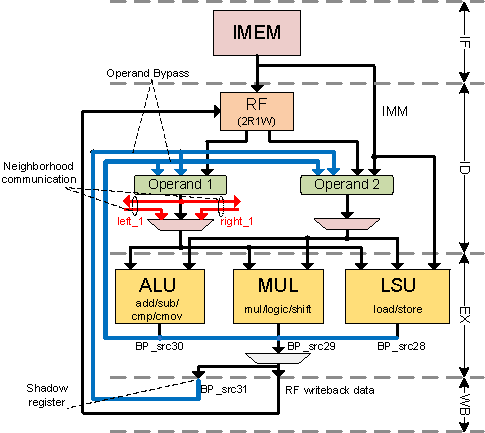
\includegraphics[width=.4\textwidth]{figures/4-stage_bypass}%
%\label{fig:4stage}}
%\hfil
%\subfloat[5-stage pipeline with explicit datapaths.]{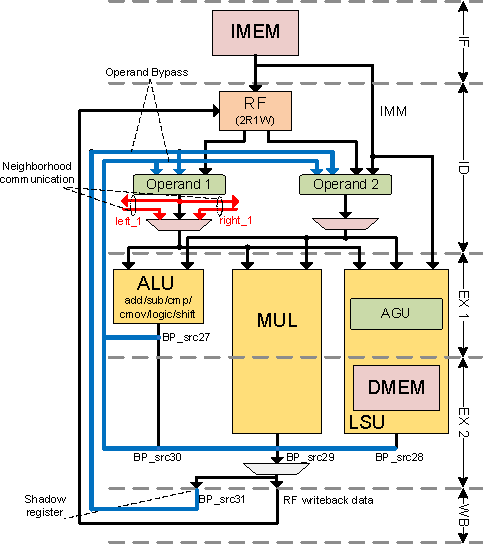
\includegraphics[width=.34\textwidth]{figures/5-stage_bypass}%
%\label{fig:5stage}}
%\caption{The pipeline of the SMD processor architecture with explicit datapaths.}
%\label{fig:pipeline_stages}
%\end{figure}

%%=============================== instruction format speech ===============================
%\section{Instruction Format}\label{sec:isa}
%%Change (optional)
%%% namely, one scalar and one vector instruction.
%%With
%%% namely, one scalar instruction that is executed on the CP, and one vector instruction that is executed on each of the PEs.
%Similar to a 2-issue VLIW instruction, an SIMD instruction consists of two subinstructions. An SIMD instruction is a 56-bit instruction that is divided up in two 28-bit subinstructions, namely, a scalar and a vector instruction. Only the CP can perform jump and branch instructions, therefore, the vector instruction can be either a R-type or an I-type instruction, while a scalar instruction can be a R-type, I-type or J-type instruction. Both sub instructions have a format, as shown in Figure \ref{fig:instruction_format}.

%\begin{figure}[H]
%\centering
%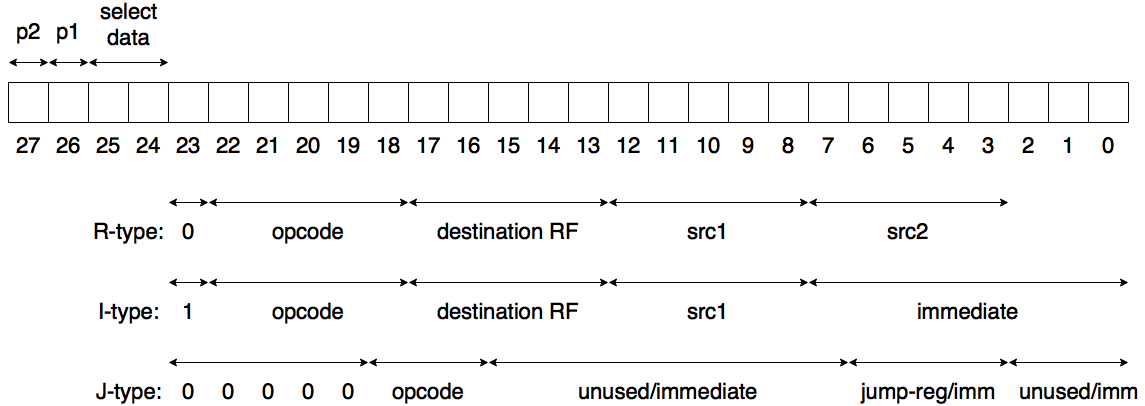
\includegraphics[width=\textwidth]{figures/instruction_format}
%\caption{Generic overview of the instruction format.}
%\label{fig:instruction_format}
%\end{figure}

%There are two guard bits $p1$ and $p2$, that can be set by using a set flag instruction. Consequently we can them for predicate execution. The instructions, branch if flag (not) set and conditional move read the predicate flag before executing. For the full overview of supported instructions, see Appendix \ref{chapter:supported_operations}.

%Note that the "select data" bits are also part of the instruction as we explained in Chapter \ref{sec:nn}. The CP and PEs can communicate by setting these bits. The communication model is shown in Table \ref{table:select_data}.
